\chapter{Quantum Trajectories.}
Often when we refer to trajectories the idea of a path comes into our minds which often is continuous in time, nevertheless, this idea is not always correct when we talk about quantum systems,  but we can keep the essence of the idea to interpret that for quantum systems a trajectory will be like the path taken by a conditional state for which the unconditional system state evolves continuously\footnote{The concept of conditional state of a system, is also know as the a-posteriori state, and it's basically the state found by using Bayesian inference. Therefore, one can infers what is happening in the system by using the readout, and is based on Bayes' theorem. From this theorem it is possible to derive that the conditional system state is given by
\[P_{X,Y}'(x|y)=\frac{P_{X,Y}(y|x)P_{X}(x)}{P_{Y}(y)}=\frac{P_{X,Y}(y|x)P_{X}(x)}{\sum_{x}P_{X,Y}(y|x)P_{X}(x)},\]
and we can also define an unconditional state by averaging over the possible measurement results as
\[P_{X}'(x)=\sum_{y}P_{X,Y}'(x|y)P_{Y}(y),\]
here the random variables $X$ and $Y$ represent the system state and the output respectevely(see the first section of \cite{Wiseman}).}.\\
The concept of quantum trajectories has provoked a huge activity in the community of quantum optics in the last years. From all this activity there has been three different interpretations of quantum trajectories: Not real, subjectively real and objectively real\cite{Wisemantrajectories}.
\subsection*{Non-Real Quantum Trajectories}
The interpretation of these ``non-real'' quantum trajectories is just simply that this formalism is just a numerical tool for solving the master equation, because computationally speaking, to solve these equations we only need $2N-2$ real numbers that have to be stored in an $N$-dimensional Hilbert space, compared to $N^{2}-1$ numbers for a state matrix.
\subsection*{Subjectively Real Quantum Trajectories}
This interpretation consider sort of degree of reality at the quantum trajectories, and the name of ``subjective reality'' s because the nature of these trajectories depend on the scheme that the observer has chosen to measure. Therefore, once the procedure of measurement has been chosen the time evolution of the conditioned system is real in the sense that for every observer the results will be the same. The subjectivity comes when we want to make an statement over a system, like for example ``an isolated exited atom will spontaneously decay at a random time'', this is not possible unless we place a photodetector to detect the emitted photon. In the case of a different procedure of measurement like heterodyne detection, we will register a continuous flow of radiation from the atom instead of a jump. Hence, the stochastic evolution of the system becomes real when the system is subject to an observation, and it is not real in an observer-less universe. 
The work done by Carmichael and co-workers \cite{Carmichaelquantum,PhysRevLett.70.2273,PhysRevLett.75.45,PhysRevA.46.R6801,Carmichael1994} was made by the motivation of the computational advantage and even though, most of their work is numerically it was possible to obtain son analytic results for son particular schemes of measurement and particular systems. There are some reasons to consider the measurement interpretation of quantum trajectories, and some of them are basically that these have opened the possibility for solve partially analytically measurement theory problems, and that subjectively real quantum trajectories give a different understanding of irreversible processes than the ones that master equation gives us.
\subsection*{Objectively Real Quantum Trajectories}
The last interpretation over quantum trajectories, consider these trajectories as independent of the measurement scheme, and this interpretation is based on the distrust of the standard interpretation of quantum mechanics, and a target to replace subjective collapses due to measurements with ``objectively real collapses'', and the roots of these approach date back to the original interpretation of the wave-function proposed by Schr\"odinger, which tries to give a real meaning of the wave-function, these interpretations are similiar to the Bohomians\cite{PratimKumar} trajectories in which the theory itself is a theory of hidden variables, which the wave-function has a representation of reality, having meaning only when irreversible processes occur. The basic problem with this ``objective'' interpretation lies with the origin of irreversible evolution. For example in optics, the master equation can be regarded as an approximation to the exact reversible evolution for the system plus its environment just as we showed in the chapter \ref{openquantumsystems}, then the problem with this interpretation is that all authors that have boarded this interpretation have not found an explanation for what is meant to be truly irreversible and what is not.\\

Here we are going to use the interpretation of ``Subjectively Real Quantum trajectories''  to describe a quantum measurement theory just as is proposed by Wiseman and Carmichael. By this approach it is possible to recreate Lindblad's equation by the simplest sort of quantum trajectories which involves a discontinuous conditioned evolution. 
\section{Continuous measurements.}
There are different approaches to describe continuous quantum measurements such as:
\begin{itemize}
\item Models of measurement.
\item Master equation
\item restricted path integrals
\item Stochastic Schr\"odinger eqution
\end{itemize}
Apart from the first one, all these ways of description are phenomenological. The conceptually most simple phenomenological approach is based upon the master equation for the density matrix, therefore, here we are going to use the ``Stochastic Scr\"odinger equation'' approach to describe continuous measurements\cite{jurgen}.\\
In order to generalise the unitary evolution of quantum states we incorporate an evolution conditioned to the measurements. Then we look for a differential equation for the density matrix state rather than the state. If we measure in an infinitesimal time, when a system it is being measured continuously (measurement time going to zero) we say that we are ``monitoring'' the system. Therefore, the evolution of the density matrix at time $t+dt$ can be obtained by averaging over all possible results
\begin{equation}
\rho(t+dt)=\sum_{r}\mathcal{J}[\hat{M}_{r}(dt)]\rho(t).
\label{quantumtrajectory1}
\end{equation}
If $\rho(t+dt)$ is differs in an infinitesimal quantity from $\rho(t)$ then we could think that at the time $dt$ we have obtained just one result ($r=0$) and set
\begin{equation}
\hat{M}_{r}(dt)=\hat{\mathbb{I}}-\left(\frac{\hat{\text{R}}}{2}+\frac{i}{\hbar}\hat{H}\right)dt,
\label{quantumtrajectory2}
\end{equation}
where $\hat{H}$ and $\hat{R}$ are Hermitian operators. However, the problem of just consider this result of measurement is that this measurement operator does not satisfy the completeness condition given in equation \eqref{Krauscompleteness} in the appendix \ref{superoperators}\footnote{As the measurement time is supposed to be infinitesimal we only preserve terms of order $dt$},
\[\hat{M}_{0}^{\dagger}(dt)\hat{M}_{0}(dt)=\hat{\mathbb{I}}-\hat{\text{R}}dt\neq \hat{\mathbb{I}}.\]
From the latter result we conclude that it's not possible to have only one measurement, because the measurement operator should be unitary\footnote{The condition of unitary is based on the fact that one can collect all information back if we would not have this condition there would be something lost and here we are assuming that everything can be recover when measured.} and as $\hat{R}\neq 0$ we need at least other possible result to fulfil the condition $\sum_r\hat{M}_r^{\dagger}(dt)\hat{M}_r(dt)$. the simplest suggestion is to consider a measurement such that $\hat{M}^{\dagger}_1(dt)\hat{M}_1(dt)=\hat{\text{R}}dt$,thus, we have that
\[\hat{M}^{\dagger}_0(dt)\hat{M}_0(dt)+\hat{M}^{\dagger}_1(dt)\hat{M}_1(dt)=\hat{\mathbb{I}},\]
which is what we wanted. Now we can consider that the possible results of measurements can be either $0$ or $1$, then we can write $\hat{\text{R}}$ and $\hat{M}_{1}(dt)$ explicitly as

\begin{align*}
\hat{M}_{1}(dt)&=\sqrt{dt}\hat{J},\\
\hat{\text{R}}&=\hat{J}^{\dagger}\hat{J},
\end{align*}
and from equation \eqref{quantumtrajectory1} we get that the evolution of $\rho$ is given by
\begin{equation}
\rho(t+dt)=\left[\hat{\mathbb{I}}-(\frac{\hat{J}^{\dagger}\hat{J}}{2}+\frac{i}{\hbar}\hat{H})dt\right]\rho(t)\left[\hat{\mathbb{I}}-(\frac{\hat{J}^{\dagger}\hat{J}}{2}-\frac{i}{\hbar}\hat{H})dt\right]+\hat{J}\rho(t)\hat{J}^{\dagger}dt,
\label{trajectory3}
\end{equation}
which has the differential form of Lindblad equation if we just take the terms of order $dt$
\begin{equation}
\dot{\rho}=-\frac{i}{\hbar}[\hat{H},\rho]+\hat{\mathcal{D}}[\hat{J}]\rho\equiv\mathcal{L}\rho.
\label{lindblad2}
\end{equation}
\section{Stochastic evolution}
As we consider above we can have two possible results of measurement $r=0,1$, then we can  compute the probability of having either $0$ or $1$ as
\[P_{1}(dt)=\text{tr}[\mathcal{J}[\hat{M}_1(dt)]\rho]=dt\text{tr}[\hat{J}^{\dagger}\hat{J}\rho],\]
\[P_{0}(dt)=1-P_1(dt).\]
Then the measurement with result $r=0$ it's considered as a null result, for this case we say that the system changes infinitesimally, but not unitarily, with the operator $\hat{M}_0(dt)$. At random times the result $r=1$ appears and this happen at rate $P_{1}(dt)/dt$ which is called a detection, and the evolution has an evolution given by the operator $\hat{M}_1(dt)$, this is what is known as a quantum jump. The interest of this case of ``quantum jumps'' is that any ``noisy trajectory'' (stochastic) can be approximate by quantum jumps.\footnote{The condition over these quantum jumps is that they have to range in size from being infinitesimal, this to guarantee that the state of the system after a jump will be always orthogonal to the one before the jump\cite{PhysRevLett.74.4827, Wiseman2002, 0305-4470-30-21-026, articlediosi}.} Nonetheless, it is important to emphasize that here this jumps represent a sudden change in the knowledge of the observer instead of an objective physical event as in Bohr's  original conception (Copenhagen interpretation)\cite{Bohr1913-BOHOTC}.\\
As we said, the evolution of the state is: either it jumps or it does not and it does it with a probability $P$ and $1-P$ respectively, this allow us then to write the evolution of the state as\footnote{See that it's necessary to normalize the state $\ket{\psi(t)}$ since we want the inner product to be orthonormal ($\bra{\psi(t)}\ket{\psi(t)}=1 \ \forall \ t$).}
\begin{equation}
\ket{\psi(t+dt)}=\left(
P\frac{\hat{M}_{1}(dt)}{\sqrt{\braket{\hat{M}_{1}^{\dagger}\hat{M}_{1}}(dt)}}+(1-P) \frac{\hat{M}_0(dt)}{\sqrt{\braket{\hat{M}_{0}^{\dagger}\hat{M}_{0}}(dt)}}\right)\ket{\psi(t)}.
\label{trajectory4}
\end{equation}
%We write it in this way in order to see that the evolution of the system can take one way  or another with probabilities $P$ and $1-P$ 
As we only have 2 possible outcomes $0$ and $1$, then the number of detections in function of time $N(t)$, then the stochastic increment $dN(t)$ must obey the following conditions\footnote{Here we are assuming that at time $t$ the state is a pure state, even though this could sound too ideal, a property of perfect monitoring is that if the system is initially in a pure state then, under perfect monitoring of its environment, this will remain in a pure state. Making then the system change its pure state in a stochastic and non-linear way.}
\begin{align}
dN(t)^{2}&=dN(t),\label{stochasticnumber}\\
\text{E}[dN(t)]&=\bra{\psi(t)}\hat{M}_{1}^{\dagger}(dt)\hat{M}_{1}(dt)\ket{\psi(t)}\equiv\braket{\hat{M}_{1}^{\dagger}(dt)\hat{M}_{1}(dt)}\nonumber\\
&=dt\bra{\psi(t)}\hat{J}^{\dagger}\hat{J}\ket{\psi(t)}dt\equiv dt\braket{\hat{J}^{\dagger}\hat{J}}(t)\label{expectedvaluedn}
\end{align} 
Let's compute now the expected value of $\hat{M}_0$\footnote{Here the expected value is the expected value over the ensemble or over the noise process.},
\[\bra{\psi(t)}\hat{M}_{0}^{\dagger}\hat{M}_{0}\ket{\psi(t)}\]

\[\bra{\psi(t)}\left(\hat{\mathbb{I}}-\frac{1}{2}\hat{J}^{\dagger}\hat{J}dt-\frac{i}{\hbar}\hat{H}dt\right)\left(\hat{\mathbb{I}}-\frac{1}{2}\hat{J}\hat{J}^{\dagger}dt+\frac{i}{\hbar}\hat{H}dt\right)\ket{\psi(t)}\]
\[\bra{\psi(t)}\hat{\mathbb{I}}-\frac{1}{2}\hat{J}dt-\frac{i}{\hbar}\hat{H}dt\hat{\mathbb{I}}-\frac{1}{2}\hat{J}dt+\frac{i}{\hbar}\hat{H}dt+O(dt^{2})\ket{\psi(t)}\]
\begin{equation}
=\bra{\psi(t)}\hat{\mathbb{I}}-\hat{J}^{\dagger}\hat{J}dt\ket{\psi(t)},
\label{expectedvaluem0}
\end{equation}
with the equation \eqref{expectedvaluem0} we can rewrite the evolution of the state $\ket{\psi}$ if the outcome is 0 as,
\begin{align}
\frac{\hat{M}_{0}(dt)}{\sqrt{\braket{\hat{M}_{0}^{\dagger}\hat{M}_{0}}(dt)}}&\approx\left(\hat{\mathbb{I}}-\frac{1}{2}\hat{J}^{\dagger}\hat{J}dt-\frac{i}{\hbar}\hat{H}dt\right)\left(1+\frac{1}{2}\braket{\hat{J}^{\dagger}\hat{J}}dt\right)\nonumber\\
&=\hat{\mathbb{I}}+\left(\frac{1}{2}\braket{\hat{J}^{\dagger}\hat{J}}-\frac{1}{2}\hat{J}^{\dagger}\hat{J}-\frac{i}{\hbar}\hat{H}\right)dt,
\label{trajectory5}
\end{align}
\begin{figure}[h!]
\centering
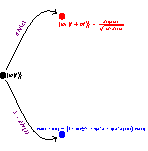
\includegraphics[width=0.7\textwidth]{Figures/equations.pdf}
\caption{Evolution of the system in the case of two possible measurements}
\label{Systemevolution}
\end{figure}  
which let us to write then the evolution of the state in terms of the stochastic differential $dN(t)$ as\footnote{Here we used the fact that $dN(t)dt$ is of higher order than $dt$ so this term can be neglect.}
\begin{align}
d\ket{\psi(t)}&=\left[\frac{\hat{M}_{1}(dt)}{\sqrt{\braket{\hat{M}_{1}^{\dagger}\hat{M}_{1}}(dt)}}-dN(t)\hat{\mathbb{I}}+\left(\frac{1}{2}\braket{\hat{J}^{\dagger}\hat{J}}-\frac{1}{2}\hat{J}^{\dagger}\hat{J}-\frac{i}{\hbar}\hat{H}\right)dt\right]\ket{\psi(t)}\nonumber\\
d\ket{\psi(t)}&=\left[\underbrace{dN(t)\left(\frac{\hat{M}_{1}(dt)}{\sqrt{\braket{\hat{M}_{1}^{\dagger}\hat{M}_{1}}(dt)}}-\hat{\mathbb{I}}\right)}_{\text{Stochastic part}}+\underbrace{dt\left(\frac{1}{2}\braket{\hat{J}^{\dagger}\hat{J}}-\frac{1}{2}\hat{J}^{\dagger}\hat{J}-\frac{i}{\hbar}\hat{H}\right)}_{\text{Deterministic part}}\right]\ket{\psi(t)}. 
\label{stochasticfashion}
\end{align}
Then as the equation \eqref{stochasticfashion} show us the evolution of the system can be expressed as one term which evolves in a deterministic way and another which give us the stochastic evolution of the system. The equation \eqref{stochasticfashion} is called stochastic mater equation and the solutions for these equations are called `\textit{Quantum trajectories} for the system.\\
In order to reconstruct the master equation, we consider a projector 
\[\hat{\Pi}(t)=\ket{\psi(t)}\bra{\psi(t)},\]
such that the expected value of this projector gives us the density matrix a time t
\begin{equation}
\text{E}[\hat{\Pi}(t)]\equiv\rho(t).
\label{projector}
\end{equation}
Just to simplify the notation we rewrite the equation \ref{stochasticfashion} as
\begin{equation}
\ket{d\psi(t)}=\ket{S(t)}dN+\ket{D(t)}dt,
\label{trajectory6}
\end{equation}
where $\ket{S(t)}$ and $\ket{D(t)}$ correspond to the stochastic and deterministic part respectively.
\[\ket{S(t)}=\left(\frac{\hat{M}_{1}(dt)}{\sqrt{\braket{\hat{M}_{1}^{\dagger}\hat{M}_{1}}(dt)}}-\hat{\mathbb{I}}\right)\ket{\psi(t)},\]
\[\ket{D(t)}=\left(\frac{1}{2}\braket{\hat{J}^{\dagger}\hat{J}}-\frac{1}{2}\hat{J}^{\dagger}\hat{J}-\frac{i}{\hbar}\hat{H}\right)\ket{\psi(t)}.\]
Then we take the differential of the projector $\hat{\Pi}(t)$and then we take the expected value and following the rules  \eqref{stochasticnumber} and \eqref{expectedvaluedn}  we derive an equation for $d\rho(t)$
\begin{align}
d\rho(t)&=\text{E}[d\hat{\Pi}(t)]=\text{E}\left[\ket{d\psi(t)}\bra{\psi(t)}+\ket{\psi(t)}\bra{d\psi(t)}+\ket{d\psi(t)}\bra{d\psi(t)}\right]\nonumber\\
&=\text{E}\left[\left(\ket{S(t)}dN+\ket{D(t)}dt\right)\bra{\psi(t)}+\ket{\psi(t)}\left(\bra{S(t)}dN+\bra{D(t)}dt\right)+\ket{S(t)}\bra{S(t)}dN\right]\nonumber\\
&=\text{E}\left[\left(\frac{\hat{J}\ket{\psi(t)}\bra{\psi(t)}\hat{J}^{\dagger}}{\braket{\hat{J}\hat{J}^{\dagger}}}-\ket{\psi(t)}\bra{\psi(t)}\right)dN+\left(\frac{i}{\hbar}\hat{H}\ket{\psi(t)}\bra{\psi(t)}-\frac{i}{\hbar}\ket{\psi(t)}\bra{\psi(t)}\hat{H}\right.\right.\nonumber\\
&\left.\left.-\frac{1}{2}\ket{\psi(t)}\bra{\psi(t)}\hat{J}^{\dagger}\hat{J}-\frac{1}{2}\hat{J}^{\dagger}\hat{J}\ket{\psi(t)}\bra{\psi(t)}+\braket{\hat{J}^{\dagger}\hat{J}}\ket{\psi(t)}\bra{\psi(t)}\right)dt\right]\nonumber\\
&=\text{E}\left[\left(\mathcal{G}[\hat{J}]dN(t)-dt\mathcal{H}\left[\frac{i}{\hbar}\hat{H}+\frac{1}{2}\hat{J}^{\dagger}\hat{J}\right]\right)\hat{\Pi}(t)\right],\label{trajectory7}
\end{align}
where the superoperators $\mathcal{G}$ and $\mathcal{H}$ are defined as
\begin{align}
\mathcal{G}[\hat{c}]\rho&=\frac{\hat{c}\rho\hat{c}^{\dagger}}{\text{tr}{\hat{c}\rho\hat{c}^{\dagger}}}-\rho, \label{superoperator1}\\
\mathcal{H}[\hat{c}]\rho&=\hat{c}\rho+\rho\hat{c}^{\dagger}-\text{tr}[\hat{c}\rho+\rho\hat{c}^{\dagger}]\rho. \label{superoperator2}
\end{align}
In order to compute the latter equation we have to use the property we have to generalise the equation \eqref{expectedvaluedn}, to calculate the expected value of the expression \eqref{trajectory7}, to do this we use a property of stochastic calculus which stablish that the way of compute an expected value of the product between a stochastic increment with expected value given by $\text{E}[dN(t)]=\lambda(X)dt$ and any function $g$ is
\begin{equation}
\text{E}[dN(t)g(\hat{\Pi}(t)]=dt\text{E}[\text{tr}[\hat{\Pi}\hat{J}^{\dagger}\hat{J}]g(\hat{\Pi}(t))],
\label{expectedvaluegeneral}
\end{equation}
then, combining the equations \eqref{trajectory7} and \eqref{expectedvaluegeneral} we get to a Lindblad's form of master equation given in \eqref{Lindbladeq}.
\begin{equation}
d\rho=-\frac{i}{\hbar}[\hat{H},\rho]dt+dt\mathcal{D}[\hat{J}]\rho.
\label{Lindbladeq2}
\end{equation}
By using the same  of argument equations \eqref{Lindbladeq2} and \eqref{stochasticfashion} can be generalised for more than just 2 possible outcomes and the these equations can be written as
\begin{equation}
\dot{\rho}=-\frac{i}{\hbar}[\hat{H},\rho]+\sum_{k}\mathcal{D}[\hat{J_{k}}]\rho,
\label{GeneralLindblad}
\end{equation}
\begin{equation}
d\ket{\psi(t)}=\sum_{k}\left[dN(t)\left(\frac{\hat{J}_{k}(dt)}{\sqrt{\braket{\hat{J}_{k}^{\dagger}\hat{J}_{k}}(dt)}}-\hat{\mathbb{I}}\right)+dt\left(\frac{1}{2}\braket{\hat{J}_{k}^{\dagger}\hat{J}_{k}}-\frac{1}{2}\hat{J}_{k}^{\dagger}\hat{J}_{k}-\frac{i}{\hbar}\hat{H}\right)\right]\ket{\psi(t)} ,
\label{Generaltrajectory}
\end{equation}
 
where $\hat{J}_{k}$ correspond to the the different operators that give the coupling between the bath and the system, these operators are also called Lindblad's operators\footnote{To check the different properties that these operators have see Appendix \ref{Lindbladappendix}.} \\


\section{Diffusive unravelings}

In every situation where a Markovian master equation can be derived, it is possible to continually measure the state of the environment, this happens if our measurements are made in a time scale large compared to the reservoir correlation time but small compared to the response time of the system.  this ``monitoring'' does not disrupt the system-reservoir coupling and the system will evolve according to the master equation, but an important situation that emerges from this is that first, the evolution of the system will follow the master equation if we ignore the results of the monitoring, however, if we take note of the results of monitoring the environment, the system will not longer obey the master equation\footnote{This is hard to understand, but as we saw in the foot note of the beginning of this chapter, if we ignore the results of the measurements we do not have knowledge certainty of the state and then we have to average over all possible outcomes whereas when we take note the uncertainty is nought since we know exactly what the state of the system is, this is the key to well understand when we refer to ``measuring ignoring the results'' and ``measuring reading the result'', and why these two have different evolution. }. 
To perfect ``monitoring'' of the environment some conditions have to be fulfilled, such as that all projective measurements have to be \textit{continual rank-one projective} well known as Von Neumann measurements or conventional measurements\footnote{Conventional measurements in quantum mechanics are defined as a collection of projector. Due to the  hermiticity of the observables, an observable $\hat{O}$ has a spectral decomposition $\hat{O}=\sum_{i}\lambda_{i}\hat{P}_{i}$ with $\hat{P}_{i}$ the projectors such that $\hat{P}_{i}\hat{P}_{j}=\hat{P}_{i}\delta_{ij}$, and $\lambda_{i}$ are unique. If $\hat{P}_{i}$ is not rank 1, it can be expressed as a sum of rank 1 projectors, this is, if the rank of $\hat{P}_{i}$ is $k$, 
\[\hat{P}_{i} =\hat{\Pi}_{1}+\hat{\Pi}_{2}+\ldots+\hat{\Pi}_{k},\]
where $\hat{\Pi}_{m}=\ket{\phi_{m}}\bra{\phi_{m}}$. Therefore, this means that projector with rank higher than 1 gives an uncertainty of the measurement since the result of the measurement will be a superposition of outcomes\cite{POVM1}\cite{POVM2}.}.
As we mentioned before the way to study quantum trajectories is via stochastic Schr\"odinger equation (SSE) which can be described as
\[\dot{\ket{\psi}}=-\frac{i}{\hbar}\hat{H}\ket{\psi}+ \text{noise}_{\psi}.\]
Although a SSE is conceptually the simplest way to define a quantum trajectory it results better if we use instead the stochastic master equation (SME), due to the invariance of the SME.\\
Assuming the initial state of the system to be pure, the quantum trajectory for its projector $\hat{\Pi}$ will be described by the SME of the form
\[\frac{d}{dt}\hat{\Pi}=\mathcal{L}\hat{\Pi}+\text{noise},\]
where the noise term is assuming to be diffusive and mean zero ($\braket{\text{noise}}=0$). By using the form of Îto calculus\footnote{A stochastic quantity $X(t)$ obeys an \^{I}to stochastic differential equation written as
\[dX=a[X(t),t)]dt+b[X(t),t]dW(t)],\]
if for all $t$ and $t_0$,
\[X(t)=X(t_0)\int_{t_{0}}^{t}dt'a[X(t'),t']+\int_{t_0}^{t}dW(t')b[X(t'),t'].\]
where $W(t)$ is a Wiener process, $X(t)$ is the variable of interest, $a[X(t),t]$ and $b[X(t),t]$ are certain known functions.\cite{StochasticNumerics}\cite{StochasticMethods}.} the latter equation can be written as
\begin{equation}
d\hat{\Pi}=\mathcal{L}\hat{\Pi}+dX,
\label{Itoform}
\end{equation}
where $dX$ is traceless, hermitian and depends linearly on the current pure state $\hat{\Pi}$ by simplicity we change $\hat{\Pi}$ by $\varrho$ to symbolise that the evolution of the projector is related with the evolution of the $\rho$ density matrix via the expected value.\\
As the SME is assumed to preserve the purity of the state the second moments of $\varrho$ are constrained by
\begin{equation}
\underbrace{d\varrho=d(\varrho^2)}_{\text{Pure state}}=\varrho d\varrho + d\varrho \varrho+d\varrho d\varrho =\underbrace{\{\varrho,d\varrho \}_{-}+d\varrho d\varrho}_{\text{Îto's calculus}},
\label{Itoscalculus}
\end{equation}
then from the equation \eqref{Itoscalculus} we see that the relation for pure states leads us to the differential relation given by Îto's calculus. This result must hold for arbitrary rank-one projectors (Von-Neumann).\\
Therefore, using Îto rules we get\footnote{In îto differentiation, one must keep all term up to second order in $dW(t)$ this means that for example if we want to compute the derivative of $\text{exp}(W(t))$ we have
\begin{align*}
d(\text{exp}(w(t))&=\text{exp}(W(t)+dW(t))-\text{exp}(W(t))=\text{exp}(W(t))\left(\text{exp}(dW(t))-1\right)\\
&=\text{exp}(W(t))\left(1+dW(t)+\frac{1}{2}dW^2(t)-1\right)=\text{exp}(W(t))\left(dW(t)+\frac{1}{2}dW^2(t)\right)
\end{align*}
It is possible to proof that $dW^2(t)=dt$ and $dW^{2+N}(t)=0$ $\forall \ N>0$.\cite{gardiner2004handbook}}
\[\mathcal{L}\varrho dt+dX=d\varrho=d(\varrho^2)=dt(\mathcal{L}\varrho)\varrho+dX\varrho+\varrho dt\mathcal{L}\varrho+\varrho dX+(dt\mathcal{L}\varrho+dX)(dt\mathcal{L}\varrho+dX)\]
\begin{equation}
=dt(\mathcal{L}\varrho)\varrho+dX\varrho+\varrho dt \mathcal{L}\varrho+\varrho dX+dXdX+dX dt\mathcal{L}\varrho+dt^2(\mathcal{L}\varrho)^2,
\label{Itolindblad1}
\end{equation}
as $dX\sim dt^{1/2}\Rightarrow dXdt\sim 0$ and $dt^2\sim 0$, then the equation \eqref{Itolindblad1} can be written as
\[dt\mathcal{L}\varrho+dX=dt\mathcal{L}\varrho \cdot\varrho+dX\varrho+\varrho dt \mathcal{L}\varrho+\varrho dX+dXdX,\]
by matching all the terms of order $dt$ and those of order $dX$,
\begin{equation}
dX=dX\varrho+\varrho dX=\{\varrho,dX\}_{+}
\label{Itolindblad2}
\end{equation}
\begin{align}
dt\mathcal{\varrho}=dt\mathcal{L}&\varrho \cdot\varrho+\varrho dt\mathcal{L}\varrho + dX dX,\nonumber\\
dXdX&=\mathcal{L}\varrho dt - dt\mathcal{L}\varrho\cdot \varrho - \varrho dt\mathcal{L}\varrho\nonumber\\
dXdX&=\mathcal{L}\varrho dt-\{\varrho,\mathcal{L}\varrho\}_{+}dt.\label{Itolindblad3}
\end{align}

A simple solution can be use as an ansatz to solve equation \eqref{Itolindblad2}
\begin{equation}
dX=\ket{d\varphi}\bra{\psi}+\ket{\psi}\bra{d\varphi}=\varrho dX+dX \varrho,
\label{ansatzitolindblad}
\end{equation}
where we have supposed that $\bra{d\varphi}\ket{\psi}=0$ and $\varrho=\ket{\psi}\bra{\psi}$, here $\ket{d\varphi}$ is an Îto differential of nought mean and is orthogonal to the current state $\ket{\psi}$.
Substituting \eqref{ansatzitolindblad} in \eqref{Itolindblad3}
\begin{align*}
&\left(\ket{d\varphi}\bra{\psi}+\ket{\psi}\bra{d\varphi}\right)\left(\ket{d\varphi}\bra{\psi}+\ket{\psi}\bra{d\varphi}\right)\\
&=\underbrace{\ket{d\varphi}\braket{\psi|d\varphi}\bra{\psi}}_{=0}+\ket{d\varphi}\underbrace{\braket{\psi|\psi}}_{=1}\bra{d\varphi}+\ket{\psi}\braket{d\varphi|d\varphi}\bra{\psi}+\underbrace{\ket{\psi}\braket{d\varphi|\psi}\bra{d\varphi}}_{=0},
\end{align*}
getting then an equation that $\ket{d\varphi}$ has to fulfil 
\begin{equation}
\ket{d\varphi}\bra{d\varphi}=\mathcal{L}\varrho dt-\{\varrho,\mathcal{L}\varrho\}_{+}dt-\ket{\psi}\braket{d\varphi|d\varphi}\bra{\psi}.
\end{equation}
To solve this equation we can use the orthogonality between the state $\ket{d\varphi}$ and $\bra{\psi}$. Multiplying by $\bra{\psi}\ldots\ket{\psi}$, it yields to
\[0=\bra{\psi}\mathcal{L}\varrho\ket{\psi}dt-\bra{\psi}\{\varrho,\mathcal{L}\varrho\}_{+}\ket{\psi}dt-\braket{d\varphi|\varphi}.\]
Expanding $\mathcal{L}\varrho$ given by equation \eqref{GeneralLindblad}, we get that the first term leads  us to
\[\bra{\psi}[\hat{H},\varrho]\ket{\psi}=\bra{\psi}\hat{H}\varrho-\varrho\hat{H}\ket{\psi}=\braket{\hat{H}}-\braket{\hat{H}}=0,\]
the second term
\begin{align*}
\bra{\psi}\hat{J}_k\varrho &\hat{J}_k^{\dagger}\ket{\psi}-\frac{1}{2}\bra{\psi}\hat{J}_k^{\dagger}\hat{J}_{k}\varrho+\varrho\hat{J}_k^{\dagger}\hat{J}_k\ket{\psi}\\
&=\braket{\hat{J}_k}\braket{\hat{J}_{k}^{\dagger}}-\frac{1}{2}\left(\braket{\hat{J}_k^{\dagger}}+\braket{\hat{J}_k^{\dagger}\hat{J}_k}\right)\\
&=\braket{\hat{J}_k}\braket{\hat{J}_{k}^{\dagger}}-\braket{\hat{J}_k^{\dagger}\hat{J}_k},
\end{align*}
Now looking at the term $\{\varrho,\mathcal{L}\varrho\}_{+}$, the part including the commutator gives us zero since $\varrho[\hat{H},\varrho]+[\hat{H},\varrho]\varrho=[\hat{H},\varrho]$, so, we look only at the other terms leading us to
\begin{align*}
\bra{\psi}\{\varrho,\mathcal{L}\varrho\}_{+}\ket{\psi}&=-\braket{\hat{J}_k^{\dagger}\hat{J}_k}-\frac{1}{2}\braket{\hat{J}_k^{\dagger}\hat{J}_k}+\braket{\hat{J}_k}\braket{\hat{J}_k^{\dagger}}-\frac{1}{2}\braket{\hat{J}_k^{\dagger}\hat{J}_k}\\
&=-2 \braket{\hat{J}_k^{\dagger}\hat{J}_k}+2\braket{\hat{J}_k}\braket{\hat{J}_k^{\dagger}},
\end{align*}
from this results we get then \cite{articlediosi2}
\begin{align}
\braket{d\varphi|d\varphi}&=\sum_{k}\left(\braket{\hat{J}_k}\braket{\hat{J}_k^{\dagger}}-2\braket{\hat{J}_k}\braket{\hat{J}_k^{\dagger}}-\braket{\hat{J}_k^{\dagger}\hat{J}_k}+2\braket{\hat{J}_k^{\dagger}\hat{J}_k}\right)dt\nonumber\\
&=\sum_{k}\left(\underbrace{\braket{\hat{J}_k^{\dagger}\hat{J}_k}-\braket{\hat{J}_k}\braket{\hat{J}_k^{\dagger}}}_{\text{Cov}(\hat{J}_k^{\dagger}\hat{J}_k)}\right)dt,
\label{Itolindblad4}
\end{align}
the latter result tell us that $\ket{d\varphi}\sim dt^{1/2}$, thus it is possible to write this in terms of a Wiener process $\xi_{k}(t)$ . To see the relation between the ``noises'' $d\xi_{k}(t)$  and the non hermitian part $\ket{d\varphi}$ we take the equation \eqref{Itolindblad4} and rewrite it as
\begin{align}
\braket{d\varphi|d\varphi}&=\sum_{kk'}\bra{\psi}\left(\hat{J}_{k'}^{\dagger}-\braket{\hat{J}_{k'}^{\dagger}}\right)\left(\hat{J}_{k}-\braket{\hat{J}_{k}}\right)\ket{\psi}d\xi_{k}^{*}d\xi_{k'}\nonumber\\
&\Rightarrow \ket{d\phi}=\sum_{k}\left(\hat{J}_{k}-\braket{\hat{J}_{k}}\right)\ket{\psi}d\xi_{k}^{*}.
\label{Itolindblad5}
\end{align}
Hence we have such that fulfils the next conditions:
\begin{itemize}
\item $\text{E}(d\xi_k(t))=0$,
\item $d\xi_{j}(t)d\xi^{*}_k(t)=\delta_{jk}dt$,
\item $d\xi_{j}(t)d\xi_{k}(t)=u_{jk}dt$,
\end{itemize}
where $u_{jk}=u_{kj}$ are arbitrary complex numbers, which are subject only to the condition that the cross-correlations for $W(t)$ are consistent with the self-correlations. this happens if and only if the vector of Wiener process $(\text{Re}[d\vec{\xi},\text{Im}[d\vec{\xi}]])$ is positive semi-definite\cite{Wiseman}
\begin{equation}
\frac{dt}{2}\begin{pmatrix}
\mathbb{I}+\text{Re}[u] & \text{Im}[u]\\
\text{Im}[u] & \mathbb{I}-\text{Re}[u]
\end{pmatrix}\geq 0.
\label{conditionoveru}
\end{equation}
The condition given in \eqref{conditionoveru} leads us to $||u||\leq 1$. So once we defined the properties of the Wiener process we have that the contribution in the change of the system is given by \eqref{Itolindblad5}, which can be interpreted as if the system jumps via the difference between operator $\hat{J}_{k}$ and its average modulated by the noise $d\xi_{k}^{*}(t)$. Finally by using the equation \eqref{ansatzitolindblad}, \eqref{Itolindblad5} and \eqref{Itoform} we get that the evolution of the density matrix is given by
\begin{equation}
d\varrho=\mathcal{L}\varrho dt+\sum_{k}\left[(\hat{J}_{k}-\braket{\hat{J}_k})\varrho d\xi^{*}_{k}(t)+\varrho(\hat{J}_k^{\dagger}-\braket{\hat{J}_k^{\dagger}})d\xi_k(t)\right].
\label{Itolindbladeq}
\end{equation}
The latter equation apply for efficient detection and can be interpreted as a state conditioned by the monitoring. To see that, it becomes necessary to consider the theory of non-projective or indirect measurement. These kind of measurements arise when the system of interest interacts with a second system which is subject to a traditional kind of measurement (projective measurement)\cite{WISEMAN200191}. In the case that the second system is initially in a pure state and a rank-on projective measurement is made on it, the indirect measurement on the system can be described by a set of operators $\Omega_{r}$ with $r$ the label of the obtained result, as in the case of the equation \eqref{quantumtrajectory1}. In order to describe the the measurement result in the infinitesimal time interval $[t,t+dt)$ we use a vector of complex numbers $\vec{I}_{k}(t)$. As a function of time, these vectorial functions are continuous but not differentiable. We are going to call these quantities ``currents'' and they are explicitly given by
\begin{equation}
I_{k}dt=\braket{u_{jk}\hat{J}_j^{\dagger}+\hat{J}_k}+d\xi_k.
\label{current}
\end{equation} 
Then it is possible to write the operator which gives the evolution of the conditioned measurement in terms of the result of the current $\vec{I}$ as\footnote{From now one we are going to use Einstein sum notation for repeated index.}
\begin{equation}
\hat{M}_{\vec{I}}=\hat{\mathbb{I}}-\frac{i}{\hbar}\hat{H}dt-\frac{1}{2}\hat{J}_k^{\dagger}\hat{J}_k dt+I^{*}_{k}\hat{J}_{k}dt.
\label{operatorcurrent}
\end{equation}
As is required by equation \eqref{Krauscompleteness} defining the operator $\hat{M}_{\vec{I}}$ as in \eqref{operatorcurrent} we need to fulfil completeness under a normalised measure $d\mu(\vec{I})$ over the space of all $\vec{I}$.
\begin{align*}
\int d\mu \hat{M}_{\vec{I}}\hat{M}_{\vec{I}}=\int d\mu \left(\hat{\mathbb{I}}-\hat{J}^{\dagger}_{k}\hat{J}_{k}dt+I_{k}\hat{J}_{k}^{\dagger}dt+I^{*}_{k}\hat{J}_{k}dt+\hat{J}_{k}\hat{J}_{j}(I_k dt)(I^{*}_k dt)\right).
\end{align*}
Then by taking the measure $d\mu$ such that
\begin{align}
\int d\mu(\vec{I})(I_k dt)&=0,\label{1conditionmu}\\
\int d\mu(\vec{I})(I^{*}_k dt)(I_{k} dt)&=\delta_{jk}dt,\label{2conditionmu}
\end{align}
The condition of completeness is fulfilled, leading us to
\[
\int d\mu(\vec{I}) \hat{M}^{\dagger}_{\vec{I}}\hat{M}_{\vec{I}}=\int d\mu (\vec{I})=\hat{\mathbb{I}}.
\]
Now let's compute the product $I_k I_j$ by computing the integral
\[\int d\mu(\vec{I})(I_k dt)(I_j dt)=\int d\mu(\vec{I}) \left(dt\braket{u_{kj}\hat{J}_{j}^{\dagger}+\hat{J}_{k}}+d\xi_k\right)\left(dt\braket{u_{jk}\hat{J}_{k}^{\dagger}+\hat{J}_{j}}+d\xi_{j}\right),\]  
keeping all terms until order of $dt$ it yields to
\begin{equation}
\int d\mu(\vec{I}) d\xi_{k}d\xi_{j}=u_{jk}dt.
\label{3conditionmu}
\end{equation}
With these relations for the measure $d\mu(\vec{I})$ we calculate the expected value of the current by calculating 
\begin{align*}
E[I_k dt]=\int d\mu(\vec{I})\Tr(\rho\hat{M}^{\dagger}_{\vec{I}}\hat{M}_{\vec{I}})I_k dt.
\end{align*}
So first we compute the trace
\begin{equation}
\Tr(\rho\hat{M}^{\dagger}_{\vec{I}}\hat{M}_{\vec{I}})=1-\left[\braket{\hat{J}^{\dagger}_{k}\hat{J}_k}+\braket{I_k\hat{J^{\dagger}_k}}+\braket{I^{*}_{k}\hat{J}_k}\right]dt,
\label{tracecurrent}
\end{equation} 
then,
\[\int d\mu(\vec{I}) \Tr(\rho\hat{M}^{\dagger}_{\vec{I}}\hat{M}_{\vec{I}})I_j=\int d \mu(\vec{I}) I_j dt +\int \braket{u_{jk}\hat{J}_{k}^{\dagger}+\hat{J}_{j}}dt d\mu(\vec{I})=\braket{u_{jk}\hat{J}_{k}^{\dagger}+\hat{J}_{j}}dt,\]
and as $E[I_k dt]=E[I_k]dt$ we finally get that the expected value of the currents is given by
\begin{equation}
E[I_k]=\braket{u_{kj}\hat{J}_{j}^{\dagger}+\hat{J}_{k}}dt.
\label{averagecurrent}
\end{equation} 
Similarly we have that the second moment of the current $I_k$ is given by
\begin{equation}
E[(I^{*}_{k}dt)(I_{j}dt)]=\delta_{jk}dt.
\label{secondmomentcurrent}
\end{equation}
So this means that with equations \eqref{averagecurrent} and \eqref{secondmomentcurrent} the currents and the noises defined above $d\xi_{k}$  they both have the same statistics.\\
The next step here is to derive the conditioned state of the system after the measurement, which is given by equation \eqref{quantumtrajectory1} by using the operator defined by \eqref{operatorcurrent}
\[\rho+d\rho_{\vec{I}}=\frac{\hat{M}_{\vec{I}}\rho\hat{M}_{\vec{I}}^{\dagger}}{\Tr[\hat{M}_{\vec{I}}\rho\hat{M}_{\vec{I}}^{\dagger}]},\]
which keeping until terms of order $dt$ leads us to
\begin{align}
d\rho_{\vec{I}}&=-\frac{1}{2}\{\hat{J}_{k}^{\dagger}\hat{J}_{k}\}_{+}dt + I_{k}^{*}dt\hat{J}_{k}\rho_{\vec{I}}\hat{J}_{j}^{\dagger}I_{j}dt+(I_{k}^{*}dtI_{k}-1)\braket{\hat{J}_{j}^{\dagger}\hat{J}_{j}}\rho_{\vec{I}}dt\nonumber\\
&-\frac{i}{\hbar}[\hat{H},\rho_{\vec{I}}]dt+\left[I^{*}_{k}(\hat{J}_{k}-\braket{\hat{J}_{k}})\rho_{\vec{I}}dt+\rho_{\vec{I}}(\hat{J}_{k}^{\dagger}-\braket{\hat{J}_{k}^{\dagger}})I_{k}dt\right]\nonumber\\
&\times\left(1-I^{*}_{j}\braket{\hat{J_{j}}}dt-I_{j}\braket{\hat{J}^{\dagger}_{j}}dt\right)
\label{evolution}
\end{align}
Substituting into the latter equation the result given by \eqref{current} it leads us to the equation \eqref{Itolindbladeq} as we expected. These results are know as a completely general dyne detection since it is possible to study via the current the behaviour of different measurements (Photo-current, Homodyne and Heterodyne detection). \\
\subsection{Invariant diffusive unravelings}
From equation \eqref{Itolindbladeq} it is possible to see that all diffusive unrevealing with $\mathbf{u}$ fixed are invariant under the shift transformation in the Hamiltonian as in the appendix \ref{Lindbladappendix}. However, from the conditions that the noise have to obey ($d\xi_j(t)d\xi_k(t)=u_{ij}dt$) it is possible to see that the unraveling is in general not invariant under unitary rearragements of the Lindblad operators  ($\hat{J}_k\rightarrow\hat{J}_l=T_{lk}\hat{J}_k$), naturally it becomes invariant if the non-Hermitian correlations $u_{jk}$ vanish. Nonetheless, in 2001 Wiseman in \cite{WISEMAN200191} proofread this idea, showing that there are more than the trivial naught non-Hermitian correlation $u_{ij}$, showing for example that for the case of finite N-dimensional Lindblad operators, which are state independent different alternatives can be chosen, for example
\begin{equation}
u_{ij}=R\Tr\left[(\hat{J}_j-N^{-1}\Tr(\hat{J}_j))(\hat{J}_k-\Tr(\hat{J}_k))\right],
\label{non-hermitiancorrelation}
\end{equation}
where $R$ is a complex number constrained only by the fact its magnitude must be sufficiently small for the positivity condition \eqref{conditionoveru} to be satisfied. For a system with unbounded Lindblad operators $\hat{J}_k$, the invariant number $R$ would have to depend on $\rho$. These correlations are trivially invariant for the shifts in the Lindblad operators, and also the fact that the correlations depend on the product $\hat{J}_k\hat{J}_j$ assures that the SME \eqref{Itolindbladeq} is under rotations (unitary transformations).\\
It is important to notice that the choice of correlations implies that the noise process $d\vec{\xi}(t)$ is no longer white, and this is because the noise correlations depend on the state of the system at that time, but as it is correlated, the noise depends on its past values of the noise. Nonetheless, the quantum trajectory defined in equation \eqref{Itolindbladeq} is Markovian, which means that the noise process is uncorrelated with $\rho$ in the case of our SME. But for example a choice of $\mathbf{u}$ would produce non-Markovian trajectories. For example taking $\mathbf{u}$ depending on the past values of the current $I$.\cite{PhysRevLett.75.4587}.
\\

With these results, in the next chapter we are going to show how via this formalism is possible to formulate Thermodynamics in a quantum regime by using the concept of a conditioned matrix state and its evolution given by the SME.




